% updates Mireille  2017 April/May 2nd 
%roles for Agents -updates  + funder
% 
In this section, we describe the currently discussed Provenance Data Model. We 
start with an UML class diagram, explain the core elements and then give 
in the following sections more details for each class and relation.
An auto-generated documentation of all classes (VO-DML compliant) is available in the Volute repository at \url{https://volute.g-vo.org/svn/trunk/projects/dm/provenance/vo-dml/ProvenanceDM.html}.

\subsection{Overview: Conceptional UML class diagram and introduction to core classes}
%We give in this section an overview on the main classes. More details about 
%each class and their relations will be explained in the following sections.
%Its core elements are colored in blue. These core elements can also be found in the W3C Provenance Data
%Model. The pattern defined by these classes is very general and can be reused everywhere where provenance is needed. 

\begin{figure}[h]
\centering
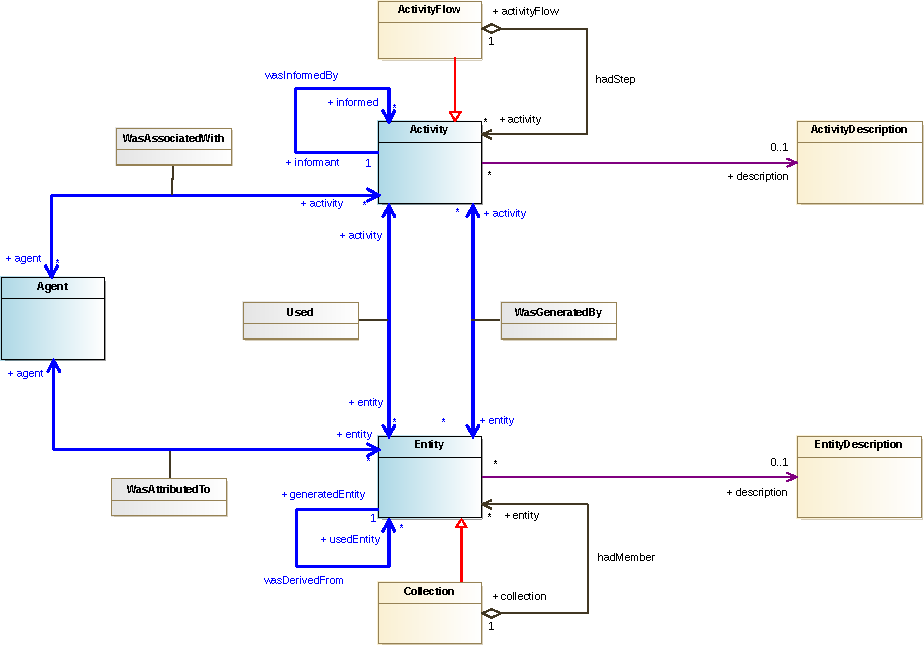
\includegraphics[width=1.0\textwidth]{../datamodel-diagrams/images/domain-classdiagram-v2.pdf}
\caption{Overview of the classes for the Provenance Data Model in a conceptual class diagram. The blue classes are core elements. There appear a number of many-to-many relationships with attached association classes (grey) which can contain additional attributes.}
%Objects in the blue box also appear in the W3C Provenance Data Model. 
%Green classes are links to the IVOA Dataset Metadata Model.}
\label{fig:classdiagram-conceptional}
\end{figure}


%\label{sec:core}
% Some examples for different use cases are given in Section \ref{sec:usecases-implementations}.
% The elements of a provenance model can be expressed as a directed graph to capture the causal dependencies. 

Figure~\ref{fig:classdiagram-conceptional} shows the conceptional UML diagram for an IVOA Provenance Data
Model.
The core elements of the Provenance Data Model are \class{Entity}, \class{Activity} and \class{Agent}. 
We chose for these elements the same names as were used in the Provenance Data 
Model of the World Wide Web Consortium (W3C, \citealt{std:W3CProvDM}), which defines 
a very abstract pattern that can be reused here. Here are the core classes with 
a short description and some examples:

\begin{itemize}
\item \class{Entity:} a thing at a certain state\\
    examples: data products like images, catalogs, parameter files, calibration data, instrument characteristics

\item \class{Activity:} an action/process or a series of actions, occurs over a period of time, performed on or caused by entities, usually results in new entities\\
    examples: data acquisition like observation, simulation; regridding, fusion, calibration steps, reconstruction

\item \class{Agent:} executes/controls an activity, is responsible for an activity or an entity\\
    examples: telescope astronomer, pipeline operator, principal investigator, software engineer, project helpdesk

\end{itemize}

\noindent



\begin{figure}[h]
\centering
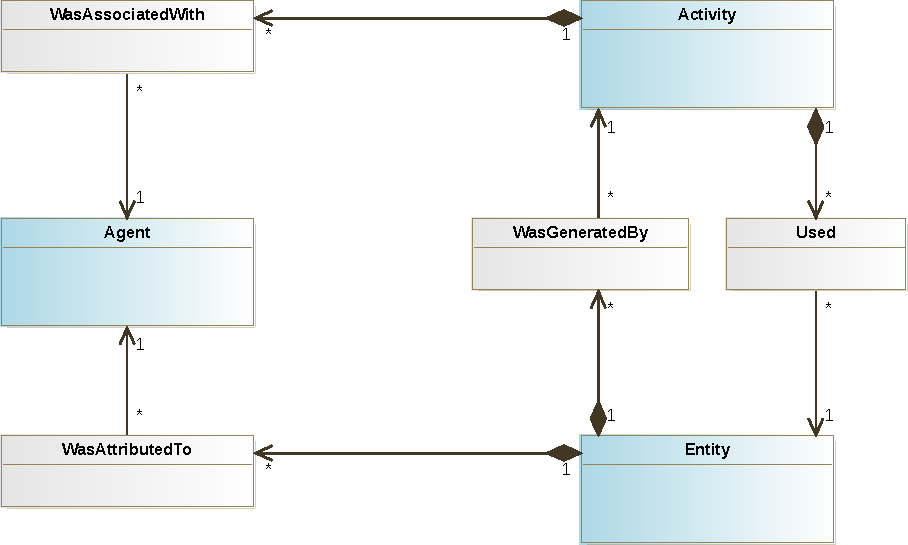
\includegraphics[scale=0.6]{../datamodel-diagrams/images/classes-core-w3c.pdf}
\caption{The main core classes and relations of the Provenance Data Model, which also occur in the W3C model.}
\label{fig:coreclasses}
\end{figure}

These core classes along with their relations to each other are provided in Figure~\ref{fig:coreclasses}.
We use the following relation classes to specify the mapping between the three core 
classes. 
The relation names were again chosen to match the W3C model names:
\begin{itemize}
\item \class{WasGeneratedBy:} a new entity is generated by an activity\\
        (entity ``image m31.fits'' wasGeneratedBy activity ``observation'')
\item \class{Used:} an entity is used by an activity\\
        (activity ``calibration'' used entities ``calibration data'', ``raw images'')
\item \class{WasAssociatedWith:} agents have responsibility for an activity\\
        (agent ``observer Max Smith'' wasAssociatedWith activity ``observation'')
\item \class{WasAttributedTo:} an entity can be attributed to an agent\\
        (entity ``image m31.fits'' wasAttributedTo ``M31 observation campaign'')
\end{itemize}

Note that the relations appear as extra classes (and thus boxes in the diagrams, instead of just having annotated relations), because they can have additional attributes -- when mapping the model to a relational database, these relations would appear as mapping tables.

In the domain of astronomy, certain processes and steps are repeated again and 
again with different parameters. We therefore separate the descriptions of activities
from the actual processes and introduce an additional \class{ActivityDescription} class (see Figure~\ref{fig:classdiagram-conceptional}).
Likewise, we also apply the same pattern for \class{Entity} and add an \class{EntityDescription}
class.
Defining such descriptions allows them to be reused, which is very useful 
when performing a series of tasks of the same type, as is typically done in 
astronomy. 

A similar normalization of descriptions of the actual processes and datasets 
can also be found in the IVOA Simulation Data Model \citep[SimDM, ][]{std:SimDM}), 
which describes simulation metadata. The SimDM classes \class{Experiment} and \class{Protocol} 
correspond to the Provenance terms \class{Activity} and \class{ActivityDescription}.

%The W3C-model has the advantage of being already an approved standard, and it 
%contains all the necessary main features needed for a Provenance model for 
%Astronomy. However, it is very general, and by adding reusable prototypes, 
%templates or descriptions for activities and entities,  the model may fit better 
%to the astronomy domain.

This separation into two classes may not be needed for each and every project,
and everyone is free to choose which classes make sense for his/her use case.
When serializing provenance, one can integrate the description side into the 
other classes, thus producing a W3C compliant provenance description. More details about 
all these classes and relations are given in the following section.


%It still remains to be seen if this separation into two classes is necessary, 
%useful or just nice to have. Currently, we include the descriptions in our model, 
%for normalization purposes. 

%But when serialising the provenance one could 
%integrate the description side into the other classes, thus producing W3C 
%compliant provenance.


\subsection{Model description}

\subsubsection{Class diagram and VO-DML compatibility}
\begin{figure}[h]
\centering
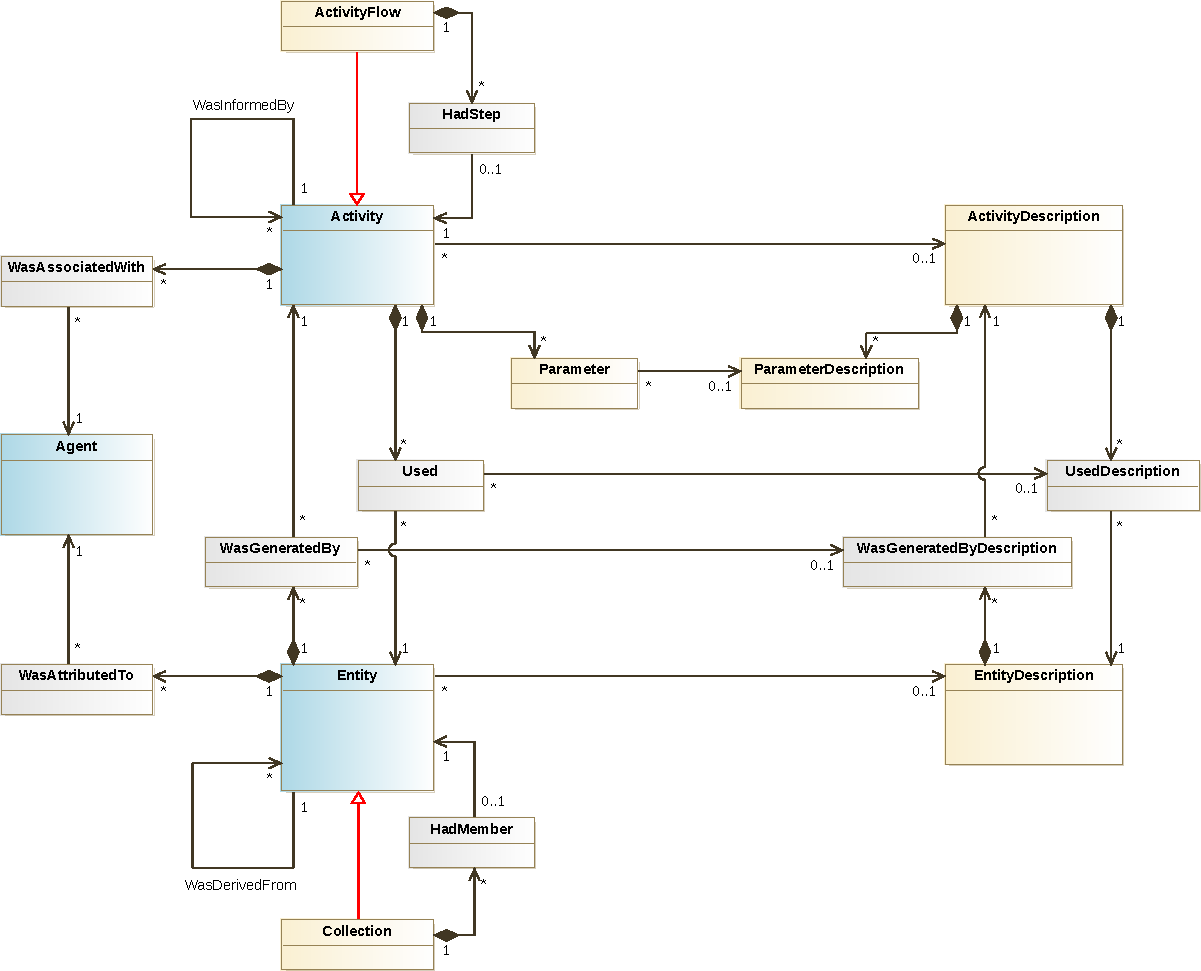
\includegraphics[width=1.0\textwidth]{../datamodel-diagrams/images/classes-overview.pdf}
\caption{More detailed overview of the classes for the Provenance Data Model. Note that this UML class diagram is more compatible with VO-DML.}
\label{fig:classdiagram}
\end{figure}

Figure~\ref{fig:classdiagram} shows the full class diagram with the association classes for the many-to-many relations modeled more directly as mapping classes. When implementing the model in a relational database, these classes can be represented as individual tables for mapping the relation. We model one of the associations of the many-to-many relationships as composition (full diamond), if the mapping class belongs more strongly to one of its linked classes, e.g. the \emph{Used} relations are strongly dependent on the corresponding \emph{Activities}. The documentation of all classes and an automatically generated figure based on the underlying xmi-description behind this UML diagram is available in the Volute repository at
\url{https://volute.g-vo.org/svn/trunk/projects/dm/provenance/vo-dml/ProvenanceDM.html}.

This version of the UML diagram is fully VO-DML compliant, i.e. we just used the restricted subset of UML to model
Provenance and reused the IVOA datatypes.


\begin{table}[h]

\small
\tymax  0.5\textwidth

\textbf{\normalsize Entity}\vspace{0.25em}\\
\begin{tabulary}{1.0\textwidth}{@{}lp{3.5cm}p{2cm}L@{}}
\toprule
\head{Attribute} & \head{W3C ProvDM} & \head{Data type} & \head{Description}\\
\midrule
\textbf{id} & prov:id & (qualified) string & a unique id for this entity (unique in its realm)\\
name       & prov:label & string & a human-readable name for the entity (to be displayed by clients)\\
type        & prov:type  & string & a provenance type, i.e. one of: prov:collection, prov:bundle, prov:plan, prov:entity; not needed for a simple entity\\
%description\_ref  & & foreign key/url & link to \class{EntityDescription}\\
annotation  & prov:description & string & text describing the entity in more detail\\
rights      & -- & string & access rights for the data, values: public, restricted or internal; can be linked to Curation.Rights from ObsCore/Dataset Metadata Model\\
creationTime  & -- & datetime & date and time at which the entity was created (e.g. timestamp of a file)\\
\midrule
\multicolumn{4}{l}{\textbf{Additional attributes:}} \\
\multicolumn{4}{l}{Further project specific attributes (e.g. size, path, url, \dots) can be added }\\
\multicolumn{4}{l}{(see Section \ref{sec:dataset-obscore})}\\
\bottomrule
\end{tabulary}
\caption{Attributes of entities. Mandatory attributes are marked in bold. Attributes from \class{EntityDescription} (see next section) may appear here as well.
}\label{tab:entity-attributes}
\end{table}


\subsubsection{Entity and EntityDescription}

Entities in astronomy are usually astronomical or astrophysical datasets in the 
form of images, tables, numbers, etc. But they can also be observation or 
simulation log files, files containing system information, environment variables, names and versions of packages, ambient conditions or, in a wider sense, also observation proposals, scientific 
articles, or manuals and other documents. 

An entity is not restricted to being a file. 
It can even be just a number in a table, depending on how fine-grained the 
provenance shall be described.

\begin{figure}[h]
\centering
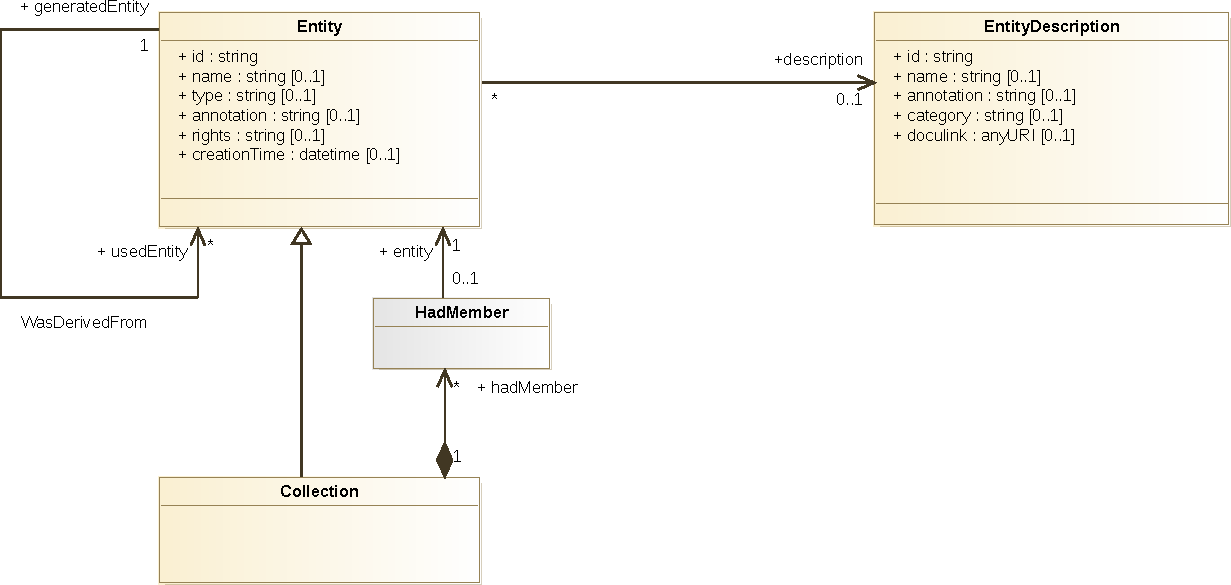
\includegraphics[scale=0.6]{../datamodel-diagrams/images/entity-details-v2.pdf}
\caption{The relation between Entity, EntityDescription and Collection (see Section~\ref{sec:collection}). 
Links to the Dataset class from the Dataset Metadata Model are described in Section~\ref{sec:dmlinks}.}
\label{fig:entity-details}
\end{figure}

The VO concept closest to Entity is the notion of ``Dataset'', which could mean a single 
table, an image or a collection of them. The Dataset Metadata Model 
\citep{std:DatasetDM} specifies an ``IVOA Dataset'' as ``a file or files which 
are considered to be a single deliverable''. 
Most attributes of the \class{Dataset} class can be mapped
directly to attributes of the \class{Entity} and EntityDescription class, see the mapping table \ref{tab:datasetmapping} in Section~\ref{sec:dmlinks}.


For entities, we suggest the attributes given in Table 
\ref{tab:entity-attributes}. If the attribute also exists in the W3C 
Provenance Data Model, we list its name in the second column.

%We discussed further attributes like \emph{size} and \emph{format}, but we decided to treat an
%entity of the same content but different format (and thus size) as the same entity,
%unless they do not have the same provenance (e.g. when the ``transformation'' activity
%for converting one format into another is included in the provenance description).

%\TODO{format and size may not be needed, if entities with the same content but different format and size are considered as the same entity.}

The difference between entities that are used as input data or output data 
becomes clear by specifying the relations between the data and activities producing or using these data.
More details on this will follow in Section \ref{sec:entity-activity-relations}.


\begin{table}[h]
\small
\tymax  0.5\textwidth
\textbf{\normalsize EntityDescription}\vspace{0.25em}\\
\begin{tabulary}{\textwidth}{@{}p{2.75cm}p{0cm}p{2cm}L@{}}
\toprule
\head{Attribute} & \head{} & \head{Data type} & \head{Description}\\
\midrule
\textbf{id} & & (qualified) string & a unique identifier for this description\\
name       & & string & a human-readable name for the entity description\\
annotation  & & string & a decriptive text for this kind of entity\\
category    & & string & specifies if the entity contains information on logging, system (environment), calibration, simulation, observation, configuration, ...\\
doculink    & & url & link to more documentation\\
% removed the obscore attributes, since specific for observations only, not applicable to configuration entities etc.
% dataproduct\_ type  & & string       & from ObsCore data model \citep{std:ObsCore}, if applicable; describes, what kind of product it is (e.g. image, table)\\
% dataproduct\_ subtype & & string       & from ObsCore data model, more specific subtype\\
% level       & & enum integer & the level of processing or calibration; for ObsCore's calib\_level it is an integer between 0 and 3\\
\midrule
\multicolumn{4}{l}{\textbf{Additional attributes:}} \\
\multicolumn{4}{l}{Further project specific attributes (e.g. format, content\_type) and/or attributes}\\
\multicolumn{4}{l}{from other data models (e.g. dataproduct\_type and -\_subtype, version, calibLevel}\\
\multicolumn{4}{l}{from DatasetDM) can be added (Section~\ref{sec:dataset-obscore})}\\
\bottomrule
\end{tabulary}
\caption{Attributes of \class{EntityDescription}. For simple use cases, 
this description class may be ignored and its attributes may be used for 
\class{Entity} instead.
%The utypes may vary depending on the data model, e.g. for simulation data they 
%would point to utypes of SimDM.
}\label{tab:entitydescription-attributes}
\end{table}


\paragraph{EntityDescription.}
%The Entity class can have an EntityDescription class attached. 
The types of entities, or datasets in astronomy, can be predefined using a description class \class{EntityDescription}.
This class is meant to store descriptive informations about an Entity that are known before the Entity instance is created. For example, if we run an activity to create a RGB image from three grey images, we may have a mandatory ``format'' for the input and output images before the execution (JPG, PNG, FITS\dots), but we probably cannot know the final ``size'' of the image  that will be created. Therefore, ``format'' would be an EntityDescription attribute , while ``size'' would be an attribute of the Entity instance. 

%This class thus stores entity-related 
Additional attributes that describe the content of the data could be derived from 
the Dataset Metadata Model (see Section \ref{sec:dataset-obscore})

The \class{EntityDescription} does NOT contain any information about the usage 
of the data, it tells nothing about them being used as input or output. This is 
defined only by the relations (and the relation descriptions) between activities
and entities (see Section \ref{sec:entity-activity-relations}).

The EntityDescription general attributes are summarized in Table 
\ref{tab:entitydescription-attributes}.



\begin{table}[h]

\small
\tymax  0.5\textwidth

\textbf{\normalsize WasDerivedFrom}\vspace{0.25em}\\
\begin{tabulary}{1.0\textwidth}{@{}lp{3cm}L@{}}
\toprule
\head{Attribute} & \head{Data type}   & \head{Description}\\
\midrule
id               & string              & a unique id for this entity (unique in its realm)\\
\textbf{generatedEntity} & string      & foreign key to the entity\\
\textbf{usedEntity}      & string      & foreign key to the progenitor, from which the generatedEntity was derived\\
activity         & string              & foreign key to the generation activity\\
generation       & string              & foreign key to the wasGeneratedBy relation\\
usage            & string              & foreign key to the used relation\\
\bottomrule
\end{tabulary}
\caption{Attributes of the WasDerivedFrom relation. This is the same as used in W3C's ProvDM. Mandatory attributes are marked in bold.
}\label{tab:wasderivedfrom-attributes}
\end{table}


\paragraph{WasDerivedFrom.}
In Figure~\ref{fig:entity-details} there is one more relation that we have not mentioned yet: 
the \class{WasDerivedFrom}-relation which links two entities together, borrowed from the W3C model. 
It is used to express that 
one entity was derived from another, i.e. it can be used to find one (or more) progenitor(s) 
of a dataset, without having to look for the activities in between. It can therefore serve as 
a shortcut.

The information this relation provides is somewhat redundant, since progenitors for entities
can be found through the links to activity and the corresponding descriptions.
Nevertheless, we include \class{WasDerivedFrom} for those cases where an explicit 
link between an entity and its progenitor is useful (e.g. for speeding up searches for 
progenitors or if the activity in between is not important).

Note that the \class{WasDerivedFrom} relation
cannot always automatically be infered from following \class{WasGeneratedBy} and \class{Used} relations alone:
If there is more than one input and more than one output of an activity, it is not clear (without 
consulting the activityDescription and entity roles in the relation-descriptions) which entity was derived from which.
Only by specifying the descriptions and roles accordingly or by adding the a \class{WasDerivedFrom} relation,
this direct derivation becomes known.



\subsubsection{Collection}\label{sec:collection}
Collections are entities that are grouped together and can be treated as one single entity. 
From the provenance point of view, they have to have the \emph{same origin}, i.e., they were 
produced by the same activity (which could also be the activity of collecting
data for a publication or similar). The term ``collection'' is 
also used in the Dataset Metadata Model for grouping datasets.
% (but with a slightly different meaning). 
As an example, a collection 
with the name `RAVE survey' could consist of a number of database tables and spectra files.

%\TODO{Do we allow empty collections? Or should collections always contain at least 1 member? (otherwise they are just prov:entities?)}

The Entity-Collection relation can be modeled using the \emph{Composite} design pattern: 
Collection is a subclass of Entity, but also an aggregation of 1 to many entities, 
which could be collections themselves. 
In order to be compliant to VO-DML, we model the membership-relation explicitly 
by including a \class{HadMember} class in our model, which is connected to the
\emph{Collection} class via a composition. It may contain an additional role attribute.

Collections are also known in the W3C model, in the same sense as used here.
The relation between entity and collection is also called ``HadMember'' in the W3C model.

An additional class \class{CollectionDescription} is only 
needed if it has different attributes than 
the \class{EntityDescription}. This class should therefore only be introduced if a use case requires it.

\paragraph{Advantages of collections:} Collections can be used to collect entities with the same provenance information together, 
    in order to hide complexity where necessary. They can be used for defining 
    different levels of detail (granularity).

%\TODO{Find a really strong use case for Collections to convince everyone that they are useful/needed.}

\subsubsection{Activity and ActivityDescription}
\label{sec:activity}

\begin{figure}[h]
\centering
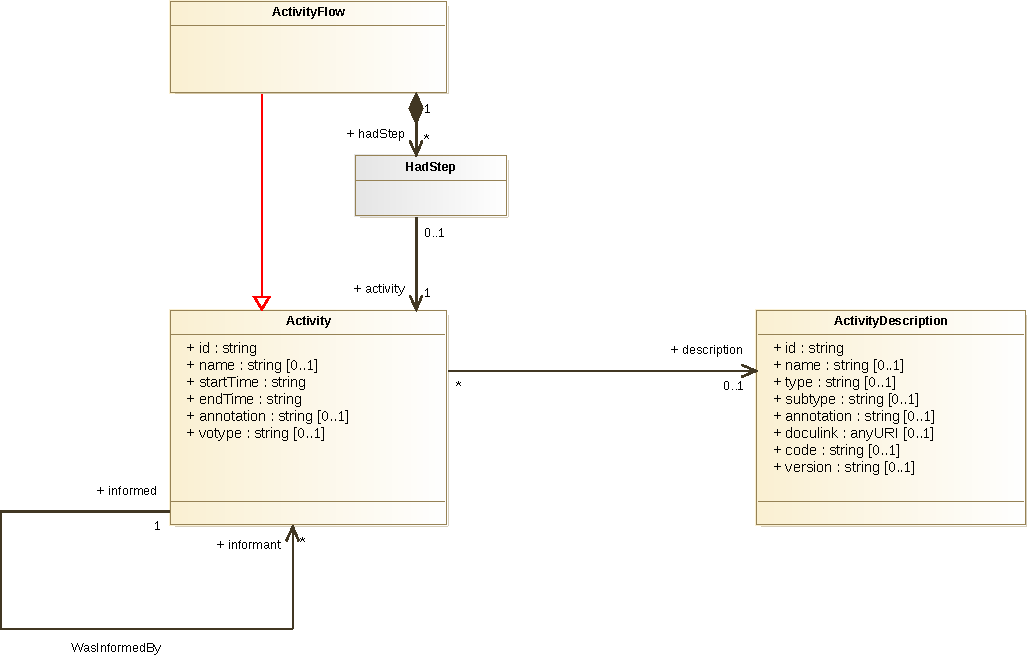
\includegraphics[scale=0.5]{../datamodel-diagrams/images/activity-details.pdf}
\caption{Details for Activity, ActivityDescription and ActivityFlow (see Section~\ref{sec:activityflow}). 
}
\label{fig:activity-details}
\end{figure}

\begin{table}[h]

\small
\tymax  0.5\textwidth

\textbf{\normalsize Activity}\vspace{0.25em}\\
\begin{tabulary}{1.0\textwidth}{@{}lp{2.5cm}p{2cm}L@{}}
\toprule
\head{Attribute} & \head{W3C ProvDM} & \head{Data type} & \head{Description}\\
\midrule
\textbf{id} & prov:id  & (qualified) string & a unique id for this activity (unique in its realm)\\
name        & prov:label  & string & a human-readable name (to be displayed by clients)\\
\textbf{startTime} & prov:startTime & datetime & start of an activity\\
\textbf{endTime} & prov:endTime  & datetime & end of an activity\\
annotation        & prov:description & string & additional explanations for the specific activity instance\\
%description\_ref  &  & foreign key/url & link to \class{ActivityDescription}\\
\bottomrule
\end{tabulary}
\caption{Attributes of \class{Activity}, their data types and equivalents in the W3C Provenance 
Data Model, if existing. Attributes in bold are \textbf{mandatory}.}
\end{table}


\begin{table}[ht]
\small
\tymax  0.5\textwidth
\textbf{\normalsize ActivityDescription}\vspace{0.25em}\\
\begin{tabulary}{1.0\textwidth}{@{}p{0cm}p{2.5cm}lL@{}}
\toprule
\head{Attribute} & \head{} & \head{Data type} & \head{Description}\\
\midrule
\textbf{id}  & & string & a unique id for this activity description (unique in its realm)\\
name         & & string & a human-readable name (to be displayed by clients)\\
type         & & string & type of the activity, from a vocabulary or list, e.g. data acquisition (observation or simulation), reduction, calibration, publication\\
subtype      & & string & more specific subtype of the activity\\
annotation  & & string & additional free text description for the activity\\
%code         & & string & the code used for this process\\
%version      & & string & a version number for the code\\
doculink     & & url    & link to further documentation on this process, e.g. a 
paper, the source code in a version control system etc.\\
\bottomrule
\end{tabulary}
\caption{Attributes of \class{ActivityDescription}.}
\end{table}


Activities in astronomy include all steps from obtaining data to the reduction of 
images and production of new datasets, like image calibration, bias subtraction, image stacking; 
light curve generation from a number of observations, radial velocity 
determination from spectra, post-processing steps of simulations etc.

\paragraph{ActivityDescription.}
The method underlying an activity can be specified by a corresponding 
\class{ActivityDescription} class (previously named \class{Method}, corresponds 
to the \class{Protocol} class in SimDM). This could be, 
for instance, the name of the code used to perform an activity or a more general 
description of the underlying algorithm or process. An activity is then a 
concrete case (instance) of using such a method, with a startTime and endTime, 
and it refers to a corresponding description for further information.

There MUST be exactly zero or one \class{ActivityDescription} per \class{Activity}. If steps from a 
pipeline shall be grouped together, one needs to create a proper 
\class{ActivityDescription} for describing all the steps at once. This method can then 
be refered to by the pipeline-activity. 

When serializing the data model, the attributes
of the description class may be assigned to the activity in order to produce 
a W3C compliant serialization (same as with Entity/EntityDescription).


\paragraph{WasInformedBy.}
The individual steps of a pipeline can be chained
together directly, without mentioning the intermediate datasets, using the \class{WasInformedBy}-relation.
This relation can be used as a short-cut, if the exchanged datasets are deemed to be not important
enough to be recorded. For grouping activities, also see the 
next section \ref{sec:activityflow}.


\subsubsection{ActivityFlow}\label{sec:activityflow}
%\TODO{Link to D-PROV!}
For facilitating grouping of activities (and their related entities etc.)
we introduce the class \class{ActivityFlow}.
It can be used for hiding and grouping a part of the workflow/pipeline 
or provenance 
description, if different levels of granularity are needed. Such pipelines and workflows are very common in astronomical data production and processing. Figure \ref{fig:provgraph-activityflow}
illustrates an example provenance graph in a detailed level (left side) 
and using the ActivityFlow (right side).


\begin{figure}[h]
\centering
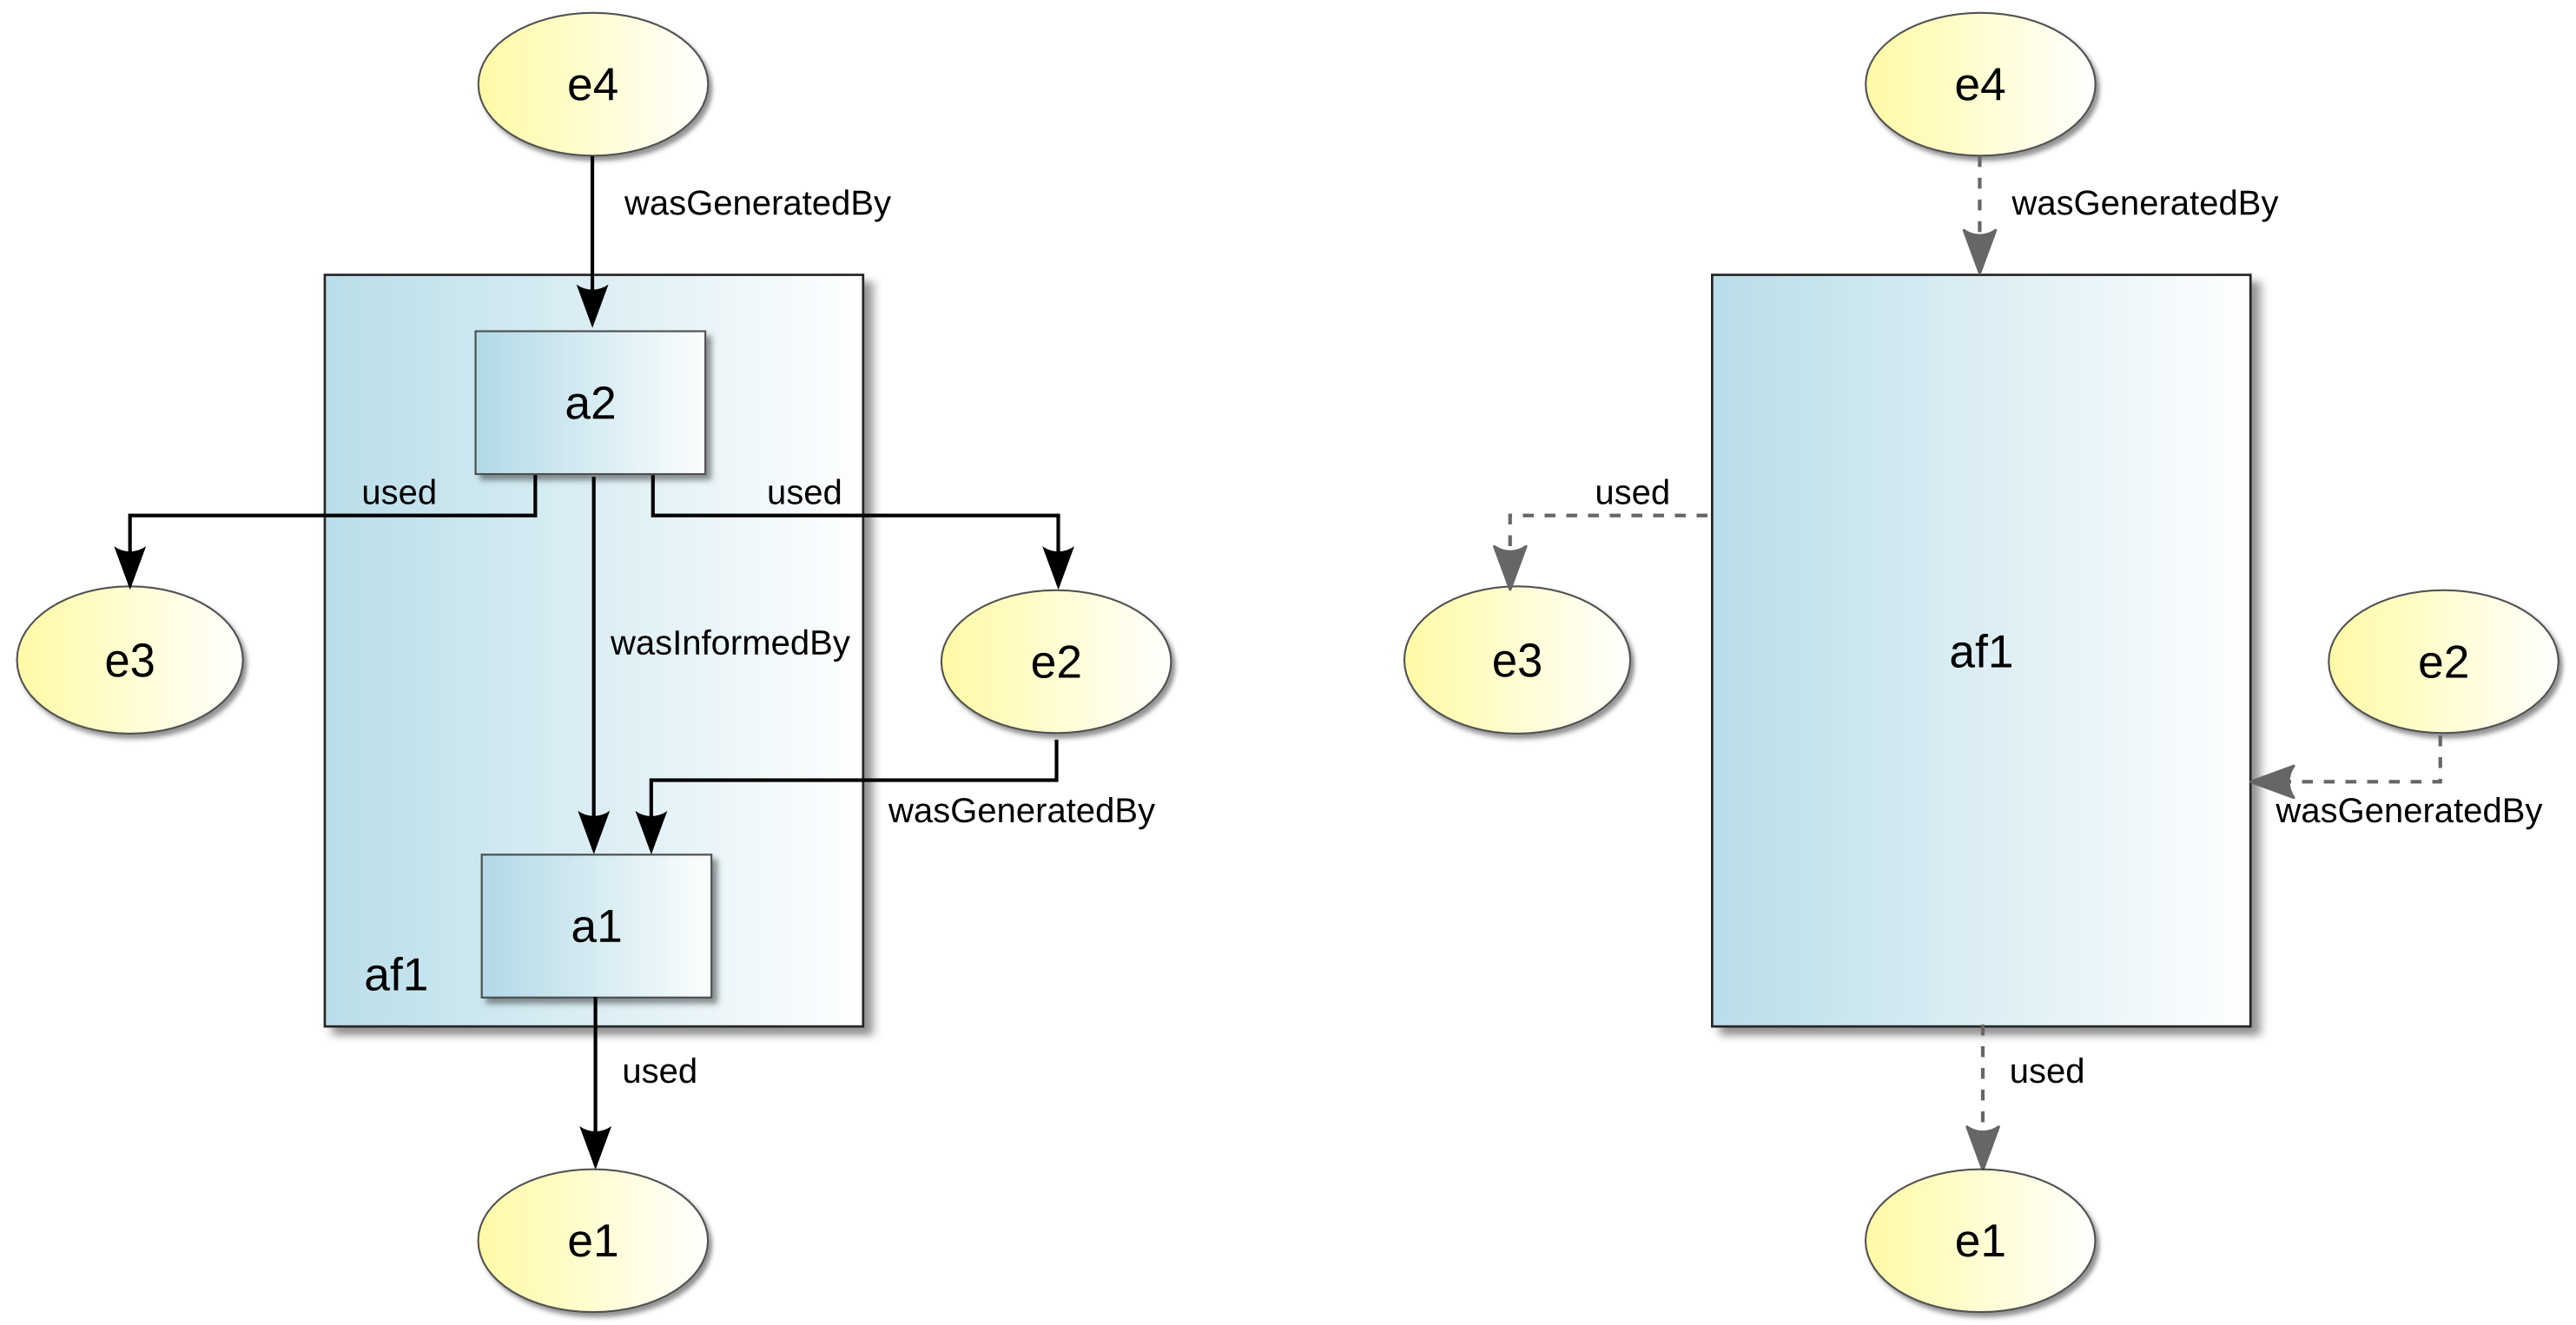
\includegraphics[width=1\textwidth]{../datamodel-diagrams/images/provgraph-activityflow}
\caption{An example provenance graph. The detailed version is shown on the left side. It also shows
the shortcut \class{WasInformedBy} to connect two activities, which could be used if the entity e2 
would not be needed anywhere else.
An ActivityFlow can be used to ``hide'' a part of the provenance graph as is shown on the right side.
Activities are marked by blue rectangles, entities by yellow ellipses.}
\label{fig:provgraph-activityflow}
\end{figure}

We also explored the different ways to describe a set of activities in the W3C 
provenance model. This model uses \class{Bundle}, i.e. an entity with type ``Bundle'', 
for wrapping a provenance description. Each part of a provenance description can be 
put into a bundle, and the bundle can then be reused in other provenance descriptions. 
W3C's \class{Plan} is an entity with type ``Plan'' and is used for describing a 
set of actions or steps. Both, \class{Bundle} and \class{Plan}, are entities and 
have the attributes and relations of this class (and thus one can define provenance of bundles and plans as well).

But we would like to consider a set of activities as being an \class{Activity} itself, 
with all the relations and properties that an activity also has. Therefore we do not reuse
W3C's classes for describing workflows and plans, but added 
the class \class{ActivityFlow} as an activity composed of activities. The composition is represented by 
the ``hadStep'' relation, as is shown in Figure~\ref{fig:activity-details}.

%while still making it obvious that this 
%group contains activities, we introduce the class \class{ActivityFlow}.
%This can be used for describing workflows or pipelines, or for 
%
%We also allow ActivityCollections to consist of a whole provenance graph of 
%activities and entities being linked together.


%We could introduce an additional abstract class, e.g. \class{AbstractActivity}, with \class{Activity} and 
%\class{ActivityFlow} being subclasses to this one. But this adds another layer of complexity 
%that we may not want in this data model.

%Since we introduced \class{ActivityFlow} mainly for having different view levels, 
%we may want to add an attribute \emph{viewLevel} to descriptions of activityflows.
% But where to set the 0 point for viewLevel???

\begin{figure}[h]
\centering
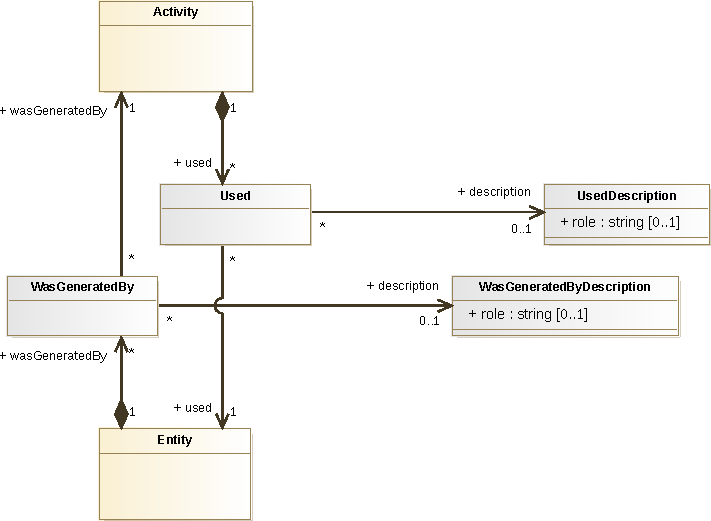
\includegraphics[scale=0.6]{../datamodel-diagrams/images/entity-activity-relations.pdf}
\hspace{0.15\textwidth}
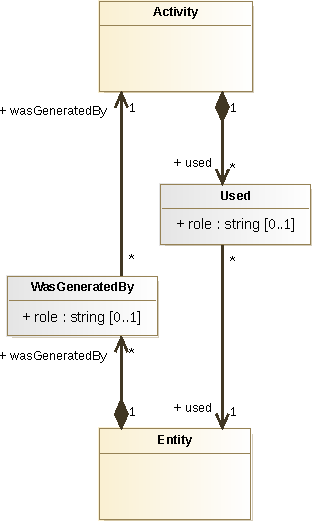
\includegraphics[scale=0.6]{../datamodel-diagrams/images/entity-activity-relations-nodesc.pdf}
\caption{\class{Entity} and \class{Activity} are linked via the \class{Used} and \class{WasGeneratedBy} relations. In the left image, the \emph{role} that an entity which was used or generated by an activity played is recorded with the corresponding \emph{UsedDescription} and \emph{WasGeneratedByDescription}, also see Section~\ref{sec:entity-roles}. If these description classes are not used, the \emph{role} can be used directly as an attribute within the \emph{Used} and \emph{WasGeneratedBy} classes (right image).}
\label{fig:entity-activity-relations}
\end{figure}


\subsubsection{Entity-Activity relations}\label{sec:entity-activity-relations}

For each data flow it should be possible to clearly identify entities and 
activities. 
%If the activities shall not be recorded explicitely, one could also 
%use the \emph{Derivation}-relation as suggested in the W3C Provenance Data Model
%to link derived entities to their originals.
Each entity is usually a result from an activity, expressed by a link from 
the entity to its generating activity using the \class{WasGeneratedBy} relation,
and can be used as input for (many) other activities, expressed by the \class{Used} relation.
Thus the information on whether data is used as input or was produced as output of 
some activity is given by the \emph{relation-types} between activities and entities.
%In fact, 
%it would be enough to provide this information just for the relations on the description side (right).
% -- Is this true?

We use two relations, \class{Used} and \class{WasGeneratedBy}, instead of just one
mapping class with a flag for input/output, because their descriptions and role-attributes
can be different. 
%in order to model the different 
%multiplicities explicitely: an entity always has only one (or none) 
%\class{WasGeneratedBy} relation, but may be \class{Used} many times as input for 
%different activities.

The \class{WasGeneratedBy}-relation can have the optional attribute \emph{time} -- this is the time, when 
the generation of the entity is finished. This generation time corresponds to e.g. \emph{DataID.date} in 
Dataset Metadata DM.
%It therefore corresponds to the \emph{created}-time used in 
%the Simulation Data Model (SimDM). 

\paragraph{Compositions and multiplicities}
In principle, an entity is produced by just one activity.
However, by introducing the \class{ActivityFlow} class for grouping activities together, 
one entity can now have many wasGeneratedBy-links to activities. One of them must 
be the actual generation activity, the other activities can only be activityFlows 
containing this generation-activity. This restriction of having only one ``true'' generation activity is not explicitly expressed in the current model\footnote{The reason for this is that we want to keep the model simple and avoid introducing even more classes.}.


The \emph{Used} relation is closely coupled to the \emph{Activity}, so we use a composition here, indicated
in Figure~\ref{fig:classdiagram} by a filled diamond: 
if an activity is deleted, then the corresponding used relations need to be removed as well. 
The entities that were used still remain, since they may have been used for other activities as well.
We need a multiplicity * between \emph{Used} and \emph{Entity}, because an entity can be used more than once
(by different activities).

Similarly, the \emph{WasGeneratedBy} relation is closely coupled with the \emph{Entity} via a composition,
since a wasGeneratedBy relation makes no sense without its entity. So if an entity is deleted, 
then its wasGeneratedBy relation must be deleted as well. There is a multiplicity * between \emph{Activity}
and \emph{WasGeneratedBy}, because an activity can generate many entities.


\paragraph{Entity roles}\label{sec:entity-roles}
Each activity requires specific roles for each input or output entity, thus 
we store this information with description classes, in the role-attributes for 
the \class{UsedDescription} and \class{WasGeneratedByDescription} relation.
For example, an activity for darkframe-subtraction requires two input images. But it is 
very important to know which of the images is the raw image and 
which one fulfils the role of dark frame.

The role is in general NOT an attribute for \class{EntityDescription} or \class{Entity}, 
since the same entity (e.g. a specific FITS file containing an image) may play 
different roles with different activities. If this is not the case, if the 
image can only play the same role everywhere, only then it is an intrinsic 
property of the entity and should be stored in the \class{EntityDescription}.

%Additionally, input (and also output) data can take different roles in an 
%activity. For example, one file could
%be a parameter file, another one is the raw image, and the third one is the 
%dark field that should be subtracted. Since these roles are very important, 
%it must be made explicit which data component needs to fulfill which role as 
%input in or output from an activity.
%Each activity requires specific roles for each input or output entity, thus 
%we store this information on the description side, in the role-attributes for 
%the \class{UsedDescription} and \class{WasGeneratedByDescription} relation.

%In W3C, this is partially solved by adding a derivation relation between the Entities (data). Here, we have a mapping-class between Activity and DataEntities as well as between ActivityDescription and DataDescription. The mapping-class at the description side, i.e. between the ActivityDescription and its DataEntityDescriptions, contains additionally a role for each relation, e.g. parameter, dark frame, raw image, etc.  If a dataset is used as input to an activity or if it results from it, will become clear with these roles.


Some example roles are given in Table \ref{tab:entity-roles}.
Note that these roles don't have to be unique, many datasets may play the same role for 
a process. For example, many image entities may be used as science-ready-images for an 
image stacking process.

\begin{table}[h]
\small
\begin{tabulary}{1.0\textwidth}{@{}lL@{}}
\toprule
\head{Role} & \head{Example entities}\\
\midrule
configuration & configuration file \\ %& used for entities that contain configuration details for an activity\\
auxiliary input & calibration image, dark frame, etc. \\%& \\
main input & raw image, science-ready images \\%& used for entities that are the main input for an activity\\
main result & image, cube or spectrum \\%& used for entities that are the main result of an activity\\
log & logging output file \\%& used for logging output \\
red & image used for red channel of a composite activity\\%& used for images that will be used as the red channel of a composite activity\\
\bottomrule
\end{tabulary}
\caption{Examples for entity roles as attributes in the 
\class{UsedDescription} and \class{WasGeneratedByDescription}.}
\label{tab:entity-roles}
\end{table}
% here we cross some notions encountered in parameter descriptions and Activity descriptions while describing parameters 

In order to facilitate interoperability, the possible 
entity-roles could be defined and described for each activity by the IVOA community, in a 
vocabulary list or thesaurus.
% TODO!!


%\TODO{Roles can be used for checking (validation) if processes use the correct type of entities, 
%e.g. check if entity-type matches used-role!}

%Without the mapping tables, the relation between \class{Activity} 
%(\class{ActivityDescription}) and \class{Entity} (\class{EntityDescription})
%would be an aggregation relation, or in other words: an association with the 
%aggregation kind ``shared''. That would be required to ensure that all 
%entities linked to an activity (either as input or output) will survive if 
%the activity is destroyed, since they are almost always shared with other 
%activities. 
%
%By using the mapping tables we make the role of an entity in an activity more 
%explicit and thus can replace the aggregation by a composition relation to the 
%\class{Activity}/\class{ActivityDescription} and simple associations to the 
%individual data components and their descriptions. 


% The derivation relation together with entities is already enough to produce a 
% Data flow view, but in astronomy we are probably even more interested in the 
% Processes (as discussed in our first draft for requirements for provenance).

%\TODO{Add an example here! (From discussions in Heidelberg.)}



\subsubsection{Parameters}\label{sec:parameters}

The concept of activity configuration, generally a set of parameters that can be configured, is different to the concept of provenance information. However, it is tightly connected. We identify three different ways to link configuration information to an activity:
\begin{itemize}
\item Declare a parameter set (or each parameter) as an input entity that is used by the activity. \\
        This also allows tracking the provenance of the parameter further.
\item Define families of activities, each one with fixed attributes.\\
        I.e. use different subclasses for activities with different fixed attributes.
\item Add activity attributes in the form of key-value parameters.
\end{itemize}

To enable the latter solution, we add a \class{Parameter} class along with a \class{ParameterDescription} for describing additional properties of activities. In this solution, Parameters are directly connected to an Activity without complex Entity-Activity relations. Moreover, we can then describe each parameter in the same way as in FIELD and PARAM elements in VOTABLE \citep{std:VOTABLE}.


\begin{table}[h]
\small
\tymax  0.5\textwidth
\textbf{\normalsize Parameter}\vspace{0.25em}\\
\begin{tabulary}{1.0\textwidth}{@{}p{0cm}p{2.5cm}lL@{}}
\toprule
\head{Attribute} & \head{} & \head{Data type} & \head{Description}\\
\midrule
\textbf{id}      & & string & parameter unique identifier\\
%description\_ref   & & foreign key/url & link to \emph{ParameterDescription}\\
%name            & & string & parameter name, if no link to ParameterDescription is given\\
\textbf{value}   & & (value dependent) & the value of the parameter\\
\bottomrule
\end{tabulary}
\caption{Attributes of \class{Parameter}. Attributes in bold are \textbf{mandatory}. Attributes of \class{ParameterDescription} can be added here as well, if that class is not used.}
\end{table}

\begin{table}[ht]
\small
\tymax  0.5\textwidth
\textbf{\normalsize ParameterDescription}\vspace{0.25em}\\
\begin{tabulary}{1.0\textwidth}{@{}p{0cm}p{2.5cm}lL@{}}
\toprule
\head{Attribute} & \head{} & \head{Data type} & \head{Description}\\
\midrule
\textbf{id}  & & string & parameter unique identifier\\
\textbf{name} & & string & parameter name\\
annotation & & string & additional free text description\\
datatype    & & string & datatype \\
unit           & & string & physical unit \\
ucd           & & string  & Unified Content Descriptor, supplying a standardized classification of the physical quantity\\
utype        & & string  & UType, meant to express the role of the parameter in the context of an external data model \\
min           & & number & minimum value \\
max           & & number & maximum value\\
options           & & list & list of accepted values\\
\bottomrule
\end{tabulary}
\caption{Attributes of \class{ParameterDescription}.}
\end{table}

For example, observations generally require information on \emph{ambient conditions} as well as 
\emph{instrument characteristics}. This contextual data associated with an observation is not directly modelled in the ProvenanceDM. However, this information can be stored as different entities. Alternatively, one could list the instrument characteristics as a set of key-value parameters using the \class{Parameter} class, so that this information is structured and stored with the provenance information (and can thus be queried simultaneously). In the case of a processing activity that cleans an image with a sigma-clipping method, the input and output images would be entities and the value of the number of sigma for sigma-clipping could be a parameter instead of an entity. We may also want to define a 3-sigma-clipping activity where this parameter is fixed to 3.


%For example for observations, the \emph{ambient conditions} as well as 
%\emph{instrument characteristics} need to be stored. But they can both be treated
%as additional entities as well. 
%Our model can then also take into account that a certain observation
%method requires special ambient conditions, already defined via the 
%ActivityDescription (e.g. radio observations rely on different ambient 
%conditions than observations
%of gamma rays), just following our data -- data description scheme.
%Ambient conditions are recorded for a certain time (startTime, endTime) and are
%usually only valid for a certain time interval. This time interval should be recorded
%with a \emph{validity}-attribute for such entities.
%
%In contrast to ambient conditions, instrument characteristics do (usually) not
%change from one observation to the other, so they are static, strictly related to
%the instrument. 
%All the characteristics could be described either as key-value pairs directly with the 
%observation (as attributes) or just as datasets, using the \class{Entity} class. 
%One would then 
%link the instrument characteristics as a type of input (or output?) dataset to a certain 
%observation activity. Thus we don't need a separate Instrument or Device class.

%\note{One should also keep in mind that some instrument related parameters can change within time,
%e.g. the CCD temperature. The instruments can also change within time because of aging.}



\subsubsection{Agent}\label{sec:w3c-agent}

An \class{Agent} describes someone who is responsible for a certain task or
entity, e.g. who pressed a button, 
ran a script, performed the observation or published a dataset.
The agent can be a single person, a group of persons (e.g. MUSE WISE Team), a 
project (CTA) or an institute. 
This is also reflected in the IVOA Dataset Metadata Model, where \class{Party} 
represents an agent, and it has two types: \class{Individual} and \class{Organization},
which are explained in more detail in Table \ref{tab:agent-types} (also see Section~\ref{sec:dmlinks} for comparison between \class{Agent} and \class{Party}).
Both agent types are also used in the W3C Provenance Data Model, though 
\class{Individual} is called \class{Person} there.
We decided to not include the type \class{SoftwareAgent} from W3C (yet), since it is not required for our current use cases. This may change in the future.

\begin{table}[h]
\small
\tymax  0.5\textwidth
\textbf{\normalsize AgentType}\vspace{0.25em}\\
\begin{tabulary}{1.0\textwidth}{@{}lllL@{}}
\toprule
\head{Class or type} & \head{W3C ProvDM} & \head{DatasetDM} &\head{Comment} \\
\midrule
Agent       & Agent  & Party & \\
Individual  & Person & Individual & a person, specified by name, email, address, 
      (though all these parts may change in time)\\
Organization & Organization & Organization & a publishing house, institute or scientific project\\


\bottomrule
\end{tabulary}
\caption{Agent class and types of agents/subclasses in this data model, compared to W3C ProvDM and DatasetDM.}
\label{tab:agent-types}
\end{table}

\begin{table}[h]
\small
\tymax  0.5\textwidth
\textbf{\normalsize Agent}\vspace{0.25em}\\
\begin{tabulary}{1.0\textwidth}{@{}llp{2cm}L@{}}
\toprule
\head{Attribute} & \head{W3C ProvDM} & \head{Data type} & \head{Description}\\
\midrule
\textbf{id} & prov:id & (qualified) string & unique identifier for an agent\\
\textbf{name} & prov:name & string & a common name for this agent; e.g. first name and last name; project name, agency name...\\
type & prov:type & string & type of the agent: either Individual (Person) or Organization\\
% insert here the attributes dedicated to contact for a Party in DataSet Metadata DM.
% \hline
% \multicolumn{4}{l}{Additional optional attributes from Dataset.Party subclasses:}\\
% \hline
% address &  & string & Address of the agent both for Individual (Person) and Organization\\
% phone   &  & string & Contact phone number of the agent both for Individual (Person) and Organization\\
% email   &  & string & Contact email of the agent both for Individual (Person) and Organization\\
\bottomrule
\end{tabulary}
\caption{Agent attributes}
\label{tab:agent-attributes}
\end{table}



A definition of organizations is given in the 
IVOA Recommendation on Resource Metadata \citep{std:ResourceMeta}, hereafter 
refered to as RM: ``An organisation is [a] specific type of resource that 
brings people together to pursue participation in VO applications.''
It also specifies further that scientific projects can be considered 
as organisations on a finer level:
``At a high level, an organisation could be a university, observatory, or government
agency. At a finer level, it could be a specific scientific project, space mission,
or individual researcher. A provider is an organisation that makes data and/or services
available to users over the network.''



For each agent a \emph{name} should be specified, a summary of the attributes for \class{Agent} is given in Table~\ref{tab:agent-attributes}.
One could also add the optional attributes \emph{address}, \emph{phone} and \emph{email} (compare with subclasses of \emph{Party} in Section~\ref{sec:dmlinks}). However, we skip them here in this main class, since an advanced system may use permanent identifiers (e.g. ORCIDs) to identify agents and retrieve their properties from an external system.
It would also increase the value of the given
information if the (current) affiliation of the agent (and a project leader/group
leader) were specified in order to maximize the chance of finding any contact 
person later on. 
The contact information is needed in case more information about a certain step in the past of a dataset is required,
but also in order
to know who was involved and to fulfill our ``Attribution'' requirement 
(Section~\ref{sec:requirements}), so that proper credits are given to the right 
people/projects. 



It is desired to have at least one agent given for each activity (and entity), but it
is not enforced.
% , hence the multiplicity between \class{Entity}/\class{Activity} and the relations
%to the \class{Agent} starts with 0.
There can also be more than one agent for each activity/entity with different \emph{roles} 
and one agent can be responsible for more than one activity or entity. This 
many-to-many relationship is made explicit in our model by adding the two
following relation classes:

\begin{itemize}
\item wasAssociatedWith: relates an \emph{activity} to an agent
\item wasAttributedTo: relates an \emph{entity} to an agent
\end{itemize}

We adopted here the same naming scheme as was used in W3C ProvDM.
Note that the attributed-to-agent for a dataset may be different from the 
agent that is associated with the activity that created an entity.
Someone who is performing a task is not necessarily given full attribution, 
especially if he acts on behalf of someone else (the project, university, ...).


\begin{table}[h]
\small
\tymax  0.5\textwidth
\textbf{\normalsize AgentRoles}\vspace{0.25em}\\
\begin{tabulary}{1.0\textwidth}{@{}lp{3cm}L@{}}
\toprule
\head{role} & \head{type or sub class} & \head{Comment} \\
\midrule
author & Individual & someone who wrote an article, software, proposal\\
contributor & Individual & someone who contributed to something (but not enough to gain authorship)\\
editor & Individual & editor of e.g. an article, before publishing\\
creator & Individual & someone who created a dataset, creators of articles or software are rather called ``author''\\
curator & Individual & someone who checked and corrected a dataset before publishing\\
publisher & Organization {(maybe also Individual?)}& organization (publishing house, institute) that published something\\
observer & Individual & observer at the telescope\\
operator & Individual & someone performing a given task \\ % removed executor: ambiguous
coordinator/PI & Individual & someone coordinating/leading a project\\ % we should choose one word : PI?
funder & Organization & agency or sponsor for a project as in Prov-N\\
provider & Organization & ``an organization that makes data and/or services available to users over the network'' (definition from RM)\\
%(owner) & voprov:Individual or voprov:Organization & Does anyone really own the data?\\
\bottomrule
\end{tabulary}
\caption{Examples for roles of agents and the typical type of that agent}
\label{tab:agent-roles}
\end{table}

%\TODO{\textbf{Mireille + Fran\c{c}ois}: Go through these roles, pick only the necessary ones, crosscheck with other data models.}



In order to make it clearer what an agent is useful for, we suggest the
possible roles an agent can have (along with descriptions partially taken from RM)
in Table~\ref{tab:agent-roles}.
For comparison, SimDM contains following roles for their contacts:
owner, creator, publisher and contributor. Note that the \emph{Party} class in Dataset and SimDM are very similar to the \emph{Agent} class, which is explained in more detail in Section~\ref{sec:dmlinks}.



This list is \emph{not} complete. We consider providing a vocabulary list for this 
in a future version of this model, collected from (future) implementations of this model.

%\TODO{Do we have a specific use case for fixing the agent-roles? Is anyone 
%going to search for specific roles in the Provenance meta-data?
%Or shall we leave it open, which roles can be defined and just give examples here?}
% ... Yes, just give examples here. Should have a vocabulary list somewhere ...

%\subsubsection{Shortcuts: WasDerivedFrom and WasInformedBy}\label{sec:shortcuts}
%The classes \class{WasDerivedFrom} and \class{WasInformedBy} can be used as ``shortcuts'' and 
%are used in the same way as the corresponding W3C classes.

%\class{WasDerivedFrom} defines the relation that links two entities together, if one entity was derived
%from the other entity. In principle, one can find this information also by tracing the 
%history of an entity backwards to the generating activity and its input entities. 
%The descriptions for activity, entity and their relations should provide enough
%information to find the progenitor entity from which an entity was derived.
%Nevertheless, we include \class{WasDerivedFrom} for those cases where an explicite 
%link between an entity and its progenitor is useful (e.g. for speeding up searches for 
%progenitors or if the activity in between is not important).

%The class \class{WasInformedBy} links two activities together without defining the
%intermediate entities that may have been exchanged. This is useful for e.g. pipelines, 
%if the intermediate entities don't play a major role or only exist temporarily, so that
%their provenance information is not deemed to be important enough to be recorded.
%``WasInformedBy'' relation (also called ``Communication'' relation, borrowed from W3C's model) 
